%
%  RULES OF THE GAME
%
%  * 80 characters
%  * line breaks at the ends of sentences
%  * eqnarrys ONLY
%  * ALWAYS cite inside parens () and use \citealt{}; no in-line cites
%  * that is all.
%

\documentclass[12pt,preprint]{aastex}

\include{vc}

\usepackage{color,hyperref}
\definecolor{linkcolor}{rgb}{0,0,0.5}
\hypersetup{colorlinks=true,linkcolor=linkcolor,citecolor=linkcolor,
            filecolor=linkcolor,urlcolor=linkcolor}
\usepackage{url}
\usepackage{amssymb,amsmath}
\usepackage{subfigure}

\newcommand{\project}[1]{{\sffamily #1}}
\newcommand{\emcee}{\project{emcee}}
\newcommand{\kepler}{\project{Kepler}}
\newcommand{\license}{MIT License}

\newcommand{\paper}{\textsl{Article}}

\newcommand{\foreign}[1]{\emph{#1}}
\newcommand{\etal}{\foreign{et\,al.}}
\newcommand{\etc}{\foreign{etc.}}

\newcommand{\Fig}[1]{Figure~\ref{fig:#1}}
\newcommand{\fig}[1]{\Fig{#1}}
\newcommand{\figlabel}[1]{\label{fig:#1}}
\newcommand{\Tab}[1]{Table~\ref{tab:#1}}
\newcommand{\tab}[1]{\Tab{#1}}
\newcommand{\tablabel}[1]{\label{tab:#1}}
\newcommand{\Eq}[1]{Equation~(\ref{eq:#1})}
\newcommand{\eq}[1]{\Eq{#1}}
\newcommand{\eqlabel}[1]{\label{eq:#1}}
\newcommand{\Sect}[1]{Section~\ref{sect:#1}}
\newcommand{\sect}[1]{\Sect{#1}}
\newcommand{\App}[1]{Appendix~\ref{sect:#1}}
\newcommand{\app}[1]{\App{#1}}
\newcommand{\sectlabel}[1]{\label{sect:#1}}

\newcommand{\dd}{\ensuremath{\,\mathrm{d}}}
\newcommand{\bvec}[1]{\ensuremath{\boldsymbol{#1}}}
\newcommand{\appropto}{\mathrel{\vcenter{
  \offinterlineskip\halign{\hfil$##$\cr
    \propto\cr\noalign{\kern2pt}\sim\cr\noalign{\kern-2pt}}}}}

% TO DOS
\newcommand{\todo}[3]{{\color{#2} \emph{#1} TODO: #3}}
\newcommand{\dfmtodo}[1]{\todo{DFM}{red}{#1}}
\newcommand{\hoggtodo}[1]{\todo{HOGG}{blue}{#1}}
\newcommand{\mortontodo}[1]{\todo{MORTON}{green}{#1}}

% Document specific variables.
\newcommand{\rate}{\ensuremath{\Gamma}}
\newcommand{\ratepar}{{\ensuremath{\theta}}}
\newcommand{\ratepars}{{\ensuremath{\bvec{\ratepar}}}}
\newcommand{\obs}[1]{\ensuremath{\hat{#1}}}
\newcommand{\radius}{\ensuremath{R}}
\newcommand{\period}{\ensuremath{P}}
\newcommand{\completeness}{{\ensuremath{P_\mathrm{c}}}}
\newcommand{\transitprob}{{\ensuremath{P_\mathrm{t}}}}
\newcommand{\data}{{\ensuremath{\bvec{x}}}}
\newcommand{\entry}{{\ensuremath{\bvec{w}}}}
\newcommand{\catalog}{{\ensuremath{\bvec{\entry}}}}

\newcommand{\interim}{{\ensuremath{\bvec{\alpha}}}}

\newcommand{\binarea}{{\ensuremath{\Delta}}}
\newcommand{\bincenter}{{\ensuremath{\bvec{x}}}}
\newcommand{\binheight}{{\ensuremath{w}}}
\newcommand{\binheights}{{\ensuremath{\bvec{\binheight}}}}

\newcommand{\mean}{{\ensuremath{\mu}}}
\newcommand{\smooth}{{\ensuremath{\lambda}}}
\newcommand{\smoothpars}{{\ensuremath{\bvec{\smooth}}}}
\newcommand{\cov}{{\ensuremath{\mathrm{K}}}}

\newcommand{\modela}{\emph{Model A}}
\newcommand{\modelb}{\emph{Model B}}

\newcommand{\gammaearth}{{\ensuremath{\rate_\oplus}}}

\begin{document}

\title{%
  Inferring the distribution and rate of Earth-like exoplanets \\
  from noisy individual-planet inferences
}

\newcommand{\nyu}{2}
\newcommand{\mpia}{3}
\newcommand{\princeton}{4}
\newcommand{\berkeley}{5}
\author{%
    Daniel~Foreman-Mackey\altaffilmark{1,\nyu},
    David~W.~Hogg\altaffilmark{\nyu,\mpia},
    Timothy~D.~Morton\altaffilmark{\princeton},
    \etal
}
\altaffiltext{1}         {To whom correspondence should be addressed:
                          \url{danfm@nyu.edu}}
\altaffiltext{\nyu}      {Center for Cosmology and Particle Physics,
                          Department of Physics, New York University,
                          4 Washington Place, New York, NY, 10003, USA}
\altaffiltext{\mpia}     {Max-Planck-Institut f\"ur Astronomie,
                          K\"onigstuhl 17, D-69117 Heidelberg, Germany}
\altaffiltext{\princeton}{Department of Astrophysics, Princeton University,
                          Princeton, NJ, 08540, USA} % CHECK THIS ZIP CODE

\begin{abstract}
Although no true extra-solar Earth analog is known, hundreds of planets have
been found around Sun-like stars that are either Earth-sized but on shorter
periods, or else on year-long orbits but somewhat bigger than Earth.
These populations ought to permit a (possibly highly uncertain) extrapolated
measurement of the probability or rate at which Sun-like stars host true Earth
analogs.
Here we present a general probabilistic framework for making justified
inferences about the occurrence rate of exoplanets taking into account survey
completeness \emph{and observational uncertainties}.
We demonstrate that our method produces lower variance estimates than the
standard inverse-detection-efficiency weighting procedure.
When applied to an existing catalog of small planet candidates around G dwarfs
(Petigura \etal\ 2013), our method confirms previous measurements of a
flattening radius distribution near Earth's radius.
One output of our models is fully marginalized estimates---marginalizing out
observational uncertainties and all distribution parameters---of the rate
density of true Earth analogs, expressed as a number of planets per star per
natural logarithmic interval of period and radius, evaluated at the properties
of Earth.
The rate density we infer is an extrapolation; it depends strongly on the
permitted flexibility of the distribution model, but it tends to come out
at around ten percent, with large uncertainty.
\end{abstract}

\keywords{%
exoplanets: sickness
---
exoplanets: eta-Earth
---
code: open-source
---
keywords: made-up-by-Hogg
}

\section{Introduction}

\hoggtodo{%
\kepler\ has been busting out exoplanets (CITE).
Many of them even appear possibly rocky and habitable (CITE).
Nonetheless, none yet known are true Earth analogs.
}

\hoggtodo{%
This hasn't stopped anyone from estimating the rate at which Sun-like stars
host Earth-like planets on year-ish period orbits (CITE).
All of these rate estimates are extrapolations of one kind or another.
Here we perform an extremely conservative extrapolation of this kind.
}

\hoggtodo{%
What would make an extrapolation like this conservative?
Using \emph{huge bins} does not a conservative estimate make.
You don't want to assume separabilities you can't justify.
You want to explore an enormous function space for the exoplanet rates or pdf.
We are going to do be conservative in these senses here, far more conservative
than anyone who has come before.
}

\dfmtodo{%
Cite \citet{tremaine} for likelihood function including multiplicity.
}

This study is novel in a number of ways.
We create probabilistic information about the full exoplanet population
\emph{not} by weighting the detected objects by the inverse detection
efficiency (\citealt{petigura}), but rather by forward modeling the
observed distribution subject to the detection efficiency
(\dfmtodo{CITE TREMAINE?} \citealt{dong}).
Re-weighting the data by inverse selection probability---a method called
V-max in the quasar and galaxy luminosity function contexts---is not wrong,
but it produces a higher-variance estimate of the population than a justified
likelihood approach; it is higher variance because
the effective number of samples, after
weighting, can be much smaller than the actual number of samples.
In this work, we build a justified
likelihood of the observed data, taking into account the completeness function
or detection efficiency.
Our likelihood function is a variable-rate Poisson likelihood; it makes the
fundamental assumption that the data points are independently drawn from the
model, but is agnostic about all other properties of the data or distribution
functions.
Indeed, the assumptions behind this study here are weaker than those of any
previous study of the period and radius distribution of the Earth-sized
exoplanet population (\dfmtodo{CITE TREMAINE?} \citealt{dong, petigura}).

Another new aspect of this study is that it makes use of very flexible
distribution function models.
Indeed most of the models we consider are ``non-parametric'' in the weak sense
that they have enormous numbers of free parameters (not the strong sense of
having an \emph{infinite} number of free parameters).
The models are protected from degeneracies and over-fitting by priors.
In some models we assume that the two-dimensional distribution of planets in
period and radius is separable; in others we don't.
We treat all of these parameters as ``nuisance parameters'' when we ask
questions about the occurrence of Earth analogs.
That is, our rate conclusions are fully marginalized, and those
marginalizations are over non-trivial numbers of parameters.

When, in what follows, we ask questions about the radius disribution of
exoplanets, the distribution parameters are no longer nuisances The
radius-distribution parameters are what we are trying to measure.
Even in this case, however, our results will have the period-distribution
parameters marginalized out.

Perhaps the most important novelty of this study is in its treatment of
observational uncertainties.
Although planet periods in our data set are very precisely measured, the
planet radius measurements have large uncertainties.
The justified probabilistic approach to including these uncertainties in a
distribution analysis is to introduce the ``true'' radii as latent variables
and infer and marginalize them out along with all other nuisance parameters.
Although this sounds expensive---and it can be---there is a simple approach
we have been advocating (\cite{hogge}) that makes use of importance sampling.
We use this approach here; our results are fully marginalized over posterior
uncertainties in all of the planet radii.
More will be said about this below; the importance sampling looks like a
product over data points of sums (averages) over individual-datum radius
samplings.

\section{A brief introduction to hierarchical inference}

In this \paper, we are asking the question: \emph{what constraints can we put
on the occurence rate of exoplanets given all the light curves measured by
\kepler?}
Mathematically, this involves evaluating the so-called \emph{marginalized
likelihood function}
\begin{eqnarray}\eqlabel{crazylike}
p(\{\data_k\}\,|\,\ratepars) &=&
    \int p(\{\data_k\}\,|\,\{\entry_k\})
    \,p(\{\entry_k\}\,|\,\ratepars)
    \dd\{\entry_k\}
\end{eqnarray}
where $\{\data_k\}$ is the set of all light curves, one light curve $\data_k$
per target $k$, \ratepars\ is a vector of parameters describing the occurence
rate function $\rate_\ratepars(\entry)$ and $\entry_k$ is the vector of
physical parameters describing the planetary system (orbital periods,
radius ratios, stellar radius, \etc) around target $k$.
In this equation, our only assumption is that the datasets depend on the
occurence rate of exoplanets only through the catalog $\{\entry_k\}$.
In our case, this assumption qualitatively means that the signals found in the
light curves depend only on the actual planet properties and not on the
distributions from which they are drawn.
It is worth noting that---as we will discuss further below---the catalog only
provides \emph{probabilistic} constraints on $\{\entry_k\}$.

In other words, a catalog is a dimensionality reduction of the raw data with
all the relevant information retained.
In the context of \kepler, the catalog reduces the set of downloaded pixel
time series (approximately 70,000 data points for the typical \kepler\ target)
to probabilistic constraints on a handful of physical parameters---\entry\
from above---like the orbital period and planetary radius.
If we take this set of parameters $\{\entry_k\}$ as \emph{sufficient
statistics} of the data then we can, in theory, compute \eq{crazylike}---up to
an unimportant constant---without ever looking at the raw data again.
This is true because the catalog provides constraints on the posterior
probability of the parameters $\{\entry_k\}$ under some choice of ``interim
prior'' \interim
\begin{eqnarray}\eqlabel{crazypost}
p(\{\entry_k\}\,|\,\{\data_k\},\,\interim) &=&
\frac{p(\{\data_k\}\,|\,\{\entry_k\})\,p(\{\entry_k\}\,|\,\interim)}
     {p(\{\data_k\}\,|\,\interim)} \quad.
\end{eqnarray}
It turns out that we can use this posterior to simplify \eq{crazylike} to a
form that can, in many common cases, be evaluated efficiently.
To find this result, multiply the integrand in \eq{crazylike} by
\begin{eqnarray}
\frac{p(\{\entry_k\}\,|\,\{\data_k\},\,\interim)}
     {p(\{\entry_k\}\,|\,\{\data_k\},\,\interim)}
\end{eqnarray}
and use \eq{crazypost} to find
\begin{eqnarray}\eqlabel{simplemarglike}
\frac{p(\{\data_k\}\,|\,\ratepars)}{p(\{\data_k\}\,|\,\interim)} &=&
    \int
    \frac{p(\{\entry_k\}\,|\,\ratepars)}{p(\{\entry_k\}\,|\,\interim)}\,
    p(\{\entry_k\}\,|\,\{\data_k\},\,\interim)
    \dd\{\entry_k\} \quad.
\end{eqnarray}
The data only enter this equation through the posterior constraints provided
by the catalog $\{\entry_k\}$!
For our purposes, this is the \emph{definition} of hierarchical inference.

The constraints in \eq{crazypost} can always be---and often are---propagated
as a list of $N$ samples $\{\entry_k^{(n)}\}$ from the posterior
\begin{eqnarray}
\{\entry_k\}^{(n)} &\sim& p(\{\entry_k\}\,|\,\{\data_k\},\,\interim) \quad.
\end{eqnarray}
We can use these samples to approximately compute the integral in
\eq{simplemarglike} as
\begin{eqnarray}\eqlabel{importance}
\frac{p(\{\data_k\}\,|\,\ratepars)}{p(\{\data_k\}\,|\,\interim)} &\approx&
    \frac{1}{N} \sum_{n=1}^N
    \frac{p(\{\entry_k^{(n)}\}\,|\,\ratepars)}
         {p(\{\entry_k^{(n)}\}\,|\,\interim)} \quad.
\end{eqnarray}
This is very efficient to compute as long as an evaluation of
$p(\{\entry_k^{(n)}\}\,|\,\ratepars)$ is not very expensive.
That being said, this could be a high variance estimator depending on the
initial choice of $p(\{\entry_k^{(n)}\}\,|\,\interim)$ but in our case, we'll
show that not many samples are needed to get an accurate estimate.

A very simple example is the familiar procedure of making a histogram.
If you model the function $p(\{\entry_k\}\,|\,\ratepars)$ as a piecewise
constant rate function---where the bin heights are the parameters---and if the
uncertainties on the catalog are negligible compared to the bin widths then
the maximum marginalized likelihood solution for \ratepars\ is a histogram of
the catalog entries (see \app{histogram} for the derivation).
The case of non-negligible uncertainties is described by \citet{hogge} using a
method similar to the one discussed here.

\section{Model generalities}

In the inference procedure described above, we only discussed an abstract
occurence rate function.
To make it more concrete, we'll model the catalog as a Poisson draw from the
\emph{observable} rate function $\obs{\rate}_\ratepars$.
This leads to the well known result (see \citealt{tabachnik,youdin} for some
of the examples from the exoplanet literature)
\begin{eqnarray}\eqlabel{poisson-like}
p(\{\entry_k\}\,|\,\ratepars) &=&
    \exp\left(-\int \obs{\rate}_\ratepars (\entry) \dd\entry\right) \,
    \prod_{k=1}^K \obs{\rate}_\ratepars (\entry_k)\quad.
\end{eqnarray}
In this equation, the integral in the normalization term is the expected
number of observable exoplanets in the sample.
A further assumption that we have made in \eq{poisson-like} is that each
object is an independent sample from the rate function.
This assumption---though it is often made---cannot be correct when we consider
systems of multiple planets.
It is possible to relax this assumption (see \citealt{tremaine} for a related
technique) but this generalization is beyond the scope of the current \paper.

The main thing to note here is that $\obs{\rate}_\ratepars$ is the rate of
exoplanets that you would expect to observe taking into account the geometric
transit probability and any other detection efficiencies.
In practice, it probably makes sense to model the observable rate as
\begin{eqnarray}
\obs{\rate}_\ratepars(\entry) &=&
    \completeness(\entry)\,\rate_\ratepars(\entry)
\end{eqnarray}
where $\completeness(\entry)$ is the detection efficiency at \entry\ and
$\rate_\ratepars(\entry)$ is the object that we want to infer: the true
occurence rate.
Up to this point, we haven't discussed any specific functional form for
$\rate_\ratepars(\entry)$ and all of this derivation is equally applicable
whether we model the occurence rate as (for example) a broken power law or
a histogram.

For the results in this \paper, we will assume that the completeness function
$\completeness(\entry)$ is known empirically but that is not a requirement for
the validity of this method.
Instead, we could use a functional form for it and infer the parameters
(\dfmtodo{cite all the papers that do the ramp, step function, whatever}).

Now, we can substitute \eq{poisson-like} into \eq{simplemarglike} and apply
the importance sampling approximation to derive the following expression for
the marginalized likelihood
\begin{eqnarray}\eqlabel{money}
\frac{p(\{\data_k\}\,|\,\ratepars)}{p(\{\data_k\}\,|\,\interim)} &\approx&
    \exp\left(-\int \obs{\rate}_\ratepars (\entry) \dd\entry\right) \,
    \prod_{k=1}^K
    \frac{1}{N_k} \sum_{n=1}^{N_k}
    \frac{\obs{\rate}_\ratepars (\entry_k^{(n)})}
         {p(\entry_k^{(n)}\,|\,\interim)} \quad.
\end{eqnarray}
In this equation, we're making the further assumption that the catalog treated
the objects independently.
In other words, we have per-object posterior samples
\begin{eqnarray}
\entry_k^{(n)} &\sim& p(\entry_k\,|\,\data_k,\,\interim) \quad.
\end{eqnarray}
\Eq{money} is the \emph{money equation} for our method.
It lets us efficiently compute the \emph{marginalized likelihood of the entire
set of light curves for a particular occurence rate function}.

\paragraph{Inverse-detection-efficiency}
It's now interesting to take a brief aside and discuss the connection between
our model and the commonly used inverse-detection-efficiency procedure
(\citealt{howard,dressing,petigura}).
This procedure involves making a weighted histogram of the catalog entries
where the weight for object $\entry_k$ is $1/\completeness(\entry_k)$.
This makes intuitive sense but (to our knowledge) does not have a clear
probabilistic justification or interpretation.

If we model the occurence rate as a histogram with $J$ fixed bin volumes
$\binarea_j$
\begin{eqnarray}
\rate_\ratepars (\entry) &=& \left\{\begin{array}{ll}
\ratepar_1 & \entry \in \binarea_1,\\
\ratepar_2 & \entry \in \binarea_2,\\
\cdots \\
\ratepar_J & \entry \in \binarea_J,\\
0 & \mathrm{otherwise}
\end{array}\right.
\end{eqnarray}
then \eq{poisson-like} becomes
\begin{eqnarray}
\ln p(\{\entry_k\}\,|\,\ratepars) &=&
    \sum_{k=1}^K \sum_{j=1}^J \mathbf{1}[\entry_k \in
        \binarea_j]\,\ln\completeness(\entry_k)\,\ratepar_j
    -\sum_{j=1}^J\ratepar_j\,\int_{\binarea_j} \completeness(\entry)\dd\entry
\end{eqnarray}
where the indicator function $\mathbf{1}[\cdot]$ is one if $\cdot$ is true and
zero otherwise.
If we take the gradient of this function with respect to \ratepars\ and set it
equal to zero, we find the maximum likelihood result
\begin{eqnarray}
\ratepar_j &=& \frac{N_j}{\int_{\binarea_j} \completeness(\entry)\dd\entry}
\end{eqnarray}
where $N_j$ is the number of objects that fall within the bin $j$.
Since it is the maximum likelihood solution, this result is the minimum
variance estimator for the occurence rate in the limit of negligible catalog
uncertainties.
This is \emph{almost} the same as the inverse-detection-efficiency result and
in various limiting cases, they would provide the same result.
\dfmtodo{Finish explaining why this result is better under the specified
assumptions.}

\paragraph{Occurence rate parameterization \& priors}
For the remainder of this \paper, we also model the occurence rate as a
two-dimensional histogram with fixed logarithmic bins in period and radius.
When we include observational uncertainties---using \eq{money}---the maximum
likelihood result is no longer analytic.
Therefore, if we want to compute the ``best-fit'' occurence rate, we can use a
standard non-linear optimization algorithm.
In the regions of parameter space that we tend to care about, the completeness
is low and there are only a few observations with large uncertainties.
In this case, we're especially interested in probabilistic constraints on the
occurence rate; not just the best-fit model.
To do this, we apply a prior\footnote{This is a slight misnomer because
we also we also marginalize over the parameters of this model.} $p(\ratepars)$
on the occurence rate parameters and generate samples from the posterior
probability
\begin{eqnarray}\eqlabel{posterior}
p(\ratepars\,|\,\{\data_k\}) &\propto&
    p(\ratepars)\,p(\{\data_k\}\,|\,\ratepars)
\end{eqnarray}
using Markov chain Monte Carlo (MCMC).

Given our model of the rate function as a collection of bins, we choose to
model the prior as a Gaussian process (\citealt{gp,gibson-gp}) on the
logarithmic bin heights.
This model encodes our prior belief that, on the grid scale that we consider,
the occurence rate should be smooth but it is otherwise very flexible about
the form of the function.
Mathematically, the prior is written as
\begin{eqnarray}
p(\ratepars) &=& p(\ratepars\,|\,\mean,\,\smooth) \\
&=& \mathcal{N} \left[\ln\ratepars;\,\mean\,\bvec{I},\,
\cov(\{\binarea_j\},\,\smoothpars)\right]
\end{eqnarray}
where $\mathcal{N}(\cdot;\,\mean\,\bvec{I},\,\cov)$ is a $J$-dimensional
Gaussian with a constant mean \mean\ and covariance matrix \cov\ that depends
on the bin locations $\{\binarea_j\}$ and a set of hyperparameters
$\smoothpars = (\smooth_0,\,\smooth_\period,\,\smooth_\radius)$.
The covariance function that we use is an anisotropic, axis-aligned
exponential-squared kernel so elements of the matrix are
\begin{eqnarray}
\cov_{ij} &=& \smooth_0\,\exp\left(-\frac{1}{2}\,
    [\binarea_i-\binarea_j]^\mathrm{T}\,\Sigma^{-1}\,[\binarea_i-\binarea_j]
\right)
\end{eqnarray}
where $\Sigma^{-1}$ is the diagonal matrix
\begin{eqnarray}
\Sigma^{-1} &=& \left(\begin{array}{cc}
1/\smooth_\period & 0 \\
0 & 1/\smooth_\radius
\end{array}\right) \quad.
\end{eqnarray}

As well as being a very flexible prior, this Gaussian process model is also
appealing because it is very well studied in the machine learning literature.
In particular, there is a very efficient algorithm---elliptical slice sampling
(ESS; \citealt{ess})---for generating samples from the posterior probability
function in \eq{posterior}.
As mentioned above, we actually go one step further and assume uniform
(hyper-)priors on $\ln\mean$ and $\ln\smoothpars$ in order to sample from the
joint posterior
\begin{eqnarray}
p(\ratepars,\,\mean,\,\smoothpars\,|\,\{\data_k\})
\end{eqnarray}
using Algorithm 1 from \citet{ess-hyper}.

For all the results below, we run a Markov chain with $10^6$ steps for the bin
heights and update the hyperparameters every 10 steps.
We discard the first \dfmtodo{XXXX} samples as burn-in and then use the
remaining samples as an approximation to the marginalized probability
distribution for \ratepars.
We tune the Metropolis--Hastings proposal used to update the hyperparameters
by hand to get an acceptance fraction of $\sim0.2-0.4$ for those parameters.

\section{Data and completeness function}

Using an independent exoplanet search and characterization pipeline,
\citet{petigura} published a catalog of 603 planet candidates orbiting stars
in their ``Sun-like'' sample of \kepler\ targets.
For each candidate, \citet{petigura} used Markov chain Monte Carlo to sample
the posterior probability density---presumably assuming uniform priors---for
the radius ratio, transit duration, and impact parameter.
They then incorporated the uncertainties in the stellar radius and published
constraints on the physical radii of their candidates.
Given this data reduction and since we don't have access to the individual
posterior constraints on radius ratio and stellar radius, we can't directly
compute the importance weights $p(\{\entry_k^\}\,|\,\interim)$ needed for
\eq{importance}.
For the rest of this \paper, we'll make the simplifying assumption that these
weights are constant in log-period and log-radius but the results don't seem
to be sensitive to this specific choice.

A huge benefit of this dataset is that Erik Petigura and collaborators
published a rigorous analysis the empirical end-to-end completeness of their
transit search pipeline.
Instead of choosing a functional form for the detection efficiency of the
pipeline as a function of the parameters of interest, \citet{petigura}
injected synthetic signals of known period and radius into the raw aperture
photometry and determining the empirical recovery rate after the full analysis.

We use all the injected samples from \citet{petigura} to compute the mean
(marginalized) detection efficiency in bins of $\ln\period$ and $\ln\radius$.
In each bin, this efficiency is simply the fraction of recovered injections.
For the purposes of this \paper, we neglect the counting uncertainties
introduced by the finite number of samples.

The largest injected signal had a radius of $16\,R_\oplus$ but, because of the
measurement uncertainties on the radii, we need to model the distribution at
larger radii.
To do this, we approximate the survey completeness for $\radius>16\,R_\oplus$
as 1.

Given our domain knowledge of how detection efficiency depends on the physical
parameters, it might seem silly to measure the survey completeness in period
and radius instead of radius ratio or signal-to-noise.
It is also likely that a change of coordinates would yield a higher precision
result.
That being said, it is still correct to measure the completeness in period and
radius, and there are a few practical reasons for our choice.
The main argument is that since the radius uncertainties are dominated by
uncertainties in the stellar parameters, it is not possible to use the
published catalog (\citealt{petigura}) to compute constraints on radius
ratios.
In future catalogs, this problem would be solved by publishing representations
of all the posterior probabilities that are being measured.
In this case, the most useful data product would be \emph{posterior samples
for each target's radius ratio and stellar radius}.

The detection efficiency also depends on the geometric transit probability
$R_\star/a$.
Since we're modeling the distribution in the period--radius plane, we need to
compute the transit probability marginalized over stellar radius and mass.
This marginalized distribution scales only with the period of the orbit as
\dfmtodo{$\propto \period^{3/2}$}.
In theory, this marginalization should be over the true distribution of these
parameters in the selected stellar catalog but we'll approximate it by
the empirical distribution.

\section{Validation using synthetic catalogs}

In order to get a feeling for the constraints provided by our method and to
explore any biases introduced by ignoring the observational uncertainties, we
start by ``observing'' a few synthetic catalogs from qualitatively different
known occurence rate functions.
For each of these simulations, we'll take the completeness function computed
by \citet{petigura} as given.
In general, \eq{poisson-like} can be sampled using a procedure called thinning
(\citealt{poisson}) but for our purposes, we'll simply consider a piecewise
constant rate function evaluated on a fine grid in log-period and log-radius.
For this discrete function, the generative procedure is simple;
\begin{enumerate}
{\item loop over each grid cell $i$,}
{\item draw Poisson random integer $K_i\sim\mathrm{Poissson}(\obs{\rate}_i)$
with the observable rate evaluated in the cell, and}
{\item distribute $K_i$ catalog entries in the cell randomly.}
\end{enumerate}
We then choose fractional observational uncertainties on the radii from the
\citet{petigura} catalog and apply them to the true catalog as Gaussian noise.

We generate synthetic catalogs from two qualitatively different rate
functions.
Both distributions are generated by a separable model
\begin{eqnarray}
\rate_\ratepars (\ln\period,\,\ln\radius) &=&
    \rate_\ratepars^{(\period)}(\ln\period)\,
    \rate_\ratepars^{(\radius)}(\ln\radius)
\end{eqnarray}
but fit using the full general model.
The first model---\modela---has a smooth occurence surface where both
distributions are smooth broken power laws.
The second---\modelb---is designed to be exactly the distribution inferred by
\citet{petigura} in the range that they considered and then smoothly
extrapolated outside that range.
The catalogs generated from these two models are shown in \fig{smooth-results}
and \fig{simulation-results}, respectively and the data are available online
at \dfmtodo{ADD SOME URL}.

For each catalog, we directly apply the inverse-detection-efficiency
procedure as implemented by \citealt{petigura}\footnote{Our implementation
exactly reproduces their results when applied to the published catalog.} and
our probabilistic method, marginalizing over the hyperparameters of the
Gaussian process regularization.
\Fig{smooth-results} and \fig{simulation-results} show the results of this
analysis in both cases.
In particular, the side panels compare the marginalized occurence rate
functions in period and radius to the true functions that were used to
generate the catalogs.
\Fig{smooth-results} shows that even if the true occurence rate is a smooth
function, the rate inferred by the inverse-detection-efficiency method can
appear to have sharp features.
In this first example---where the true distribution is well described by our
Gaussian process model---the probabilistic inference of the occurence rate is
both more precise and accurate.

In the second example, the true rate function includes a sharp feature chosen
to reproduce the result published by \citet{petigura}.
In this case, \fig{simulation-results} shows that the probabilistic
constraints on the occurence rate are less precise \emph{but more accurate}
than results using the inverse-detection-efficiency method.
At this point, the distributions inferred by these two different techniques
don't seem drastically inconsistent but the difference are most obvious as the
survey completeness goes to zero: exactly the region of interest.

\begin{figure}[p]
\begin{center}
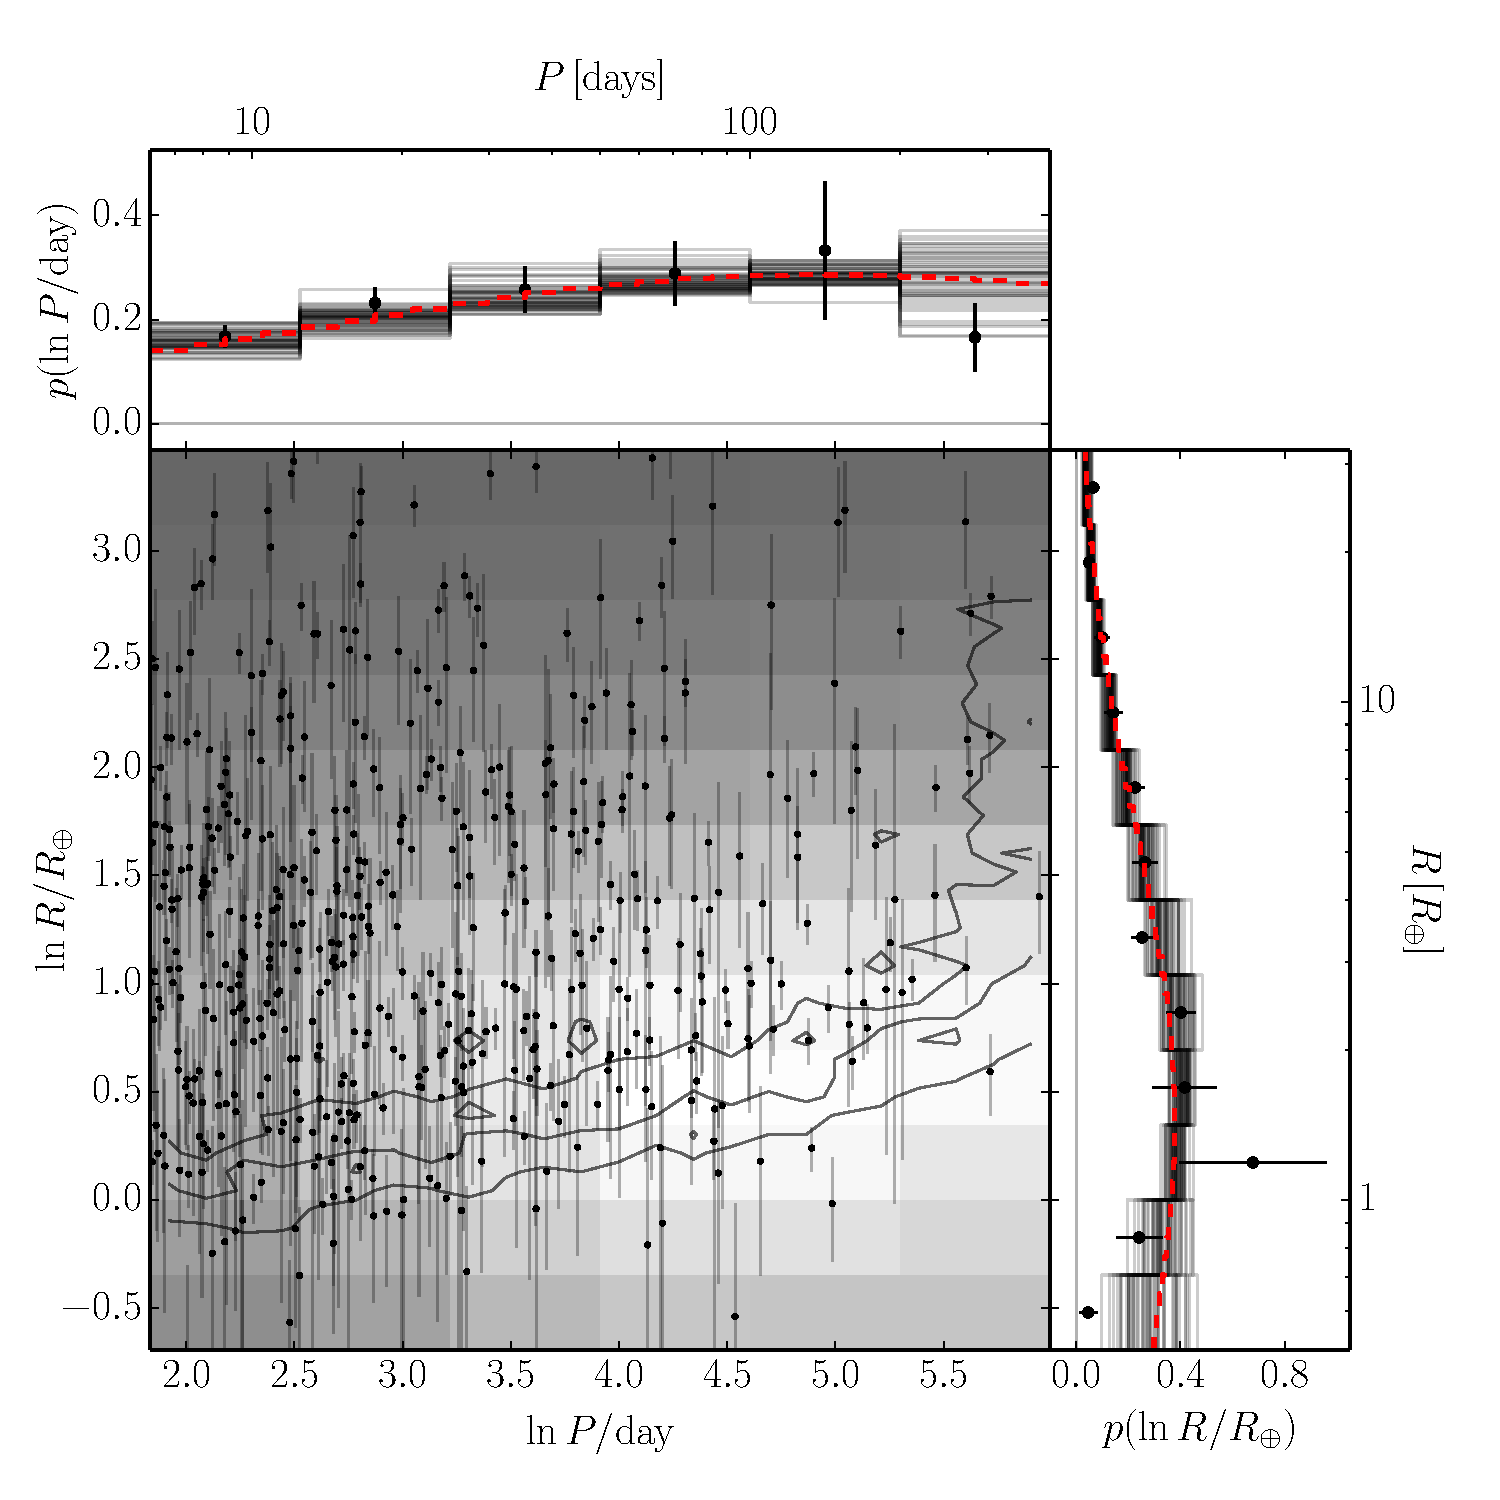
\includegraphics[width=\textwidth]{figures/smooth/results.pdf}
\end{center}
\caption{%
Inferences about the occurence rate function based on the simulated catalog
\modela.
\emph{Center:} the points with error bars show the exoplanet candidates in the
simulated incomplete catalog, the contours show the survey completeness
function (\citealt{petigura}), and the grayscale shows the median posterior
occurence surface.
\emph{Top and left:} the red dashed line shows the \emph{true} distribution
that was used to generate the catalog, the points with error bars show the
results of the inverse-detection-efficiency procedure, and the histograms are
posterior samples from the marginalized occurence rate as inferred by our
method.
\figlabel{smooth-results}}
\end{figure}

\begin{figure}[p]
\begin{center}
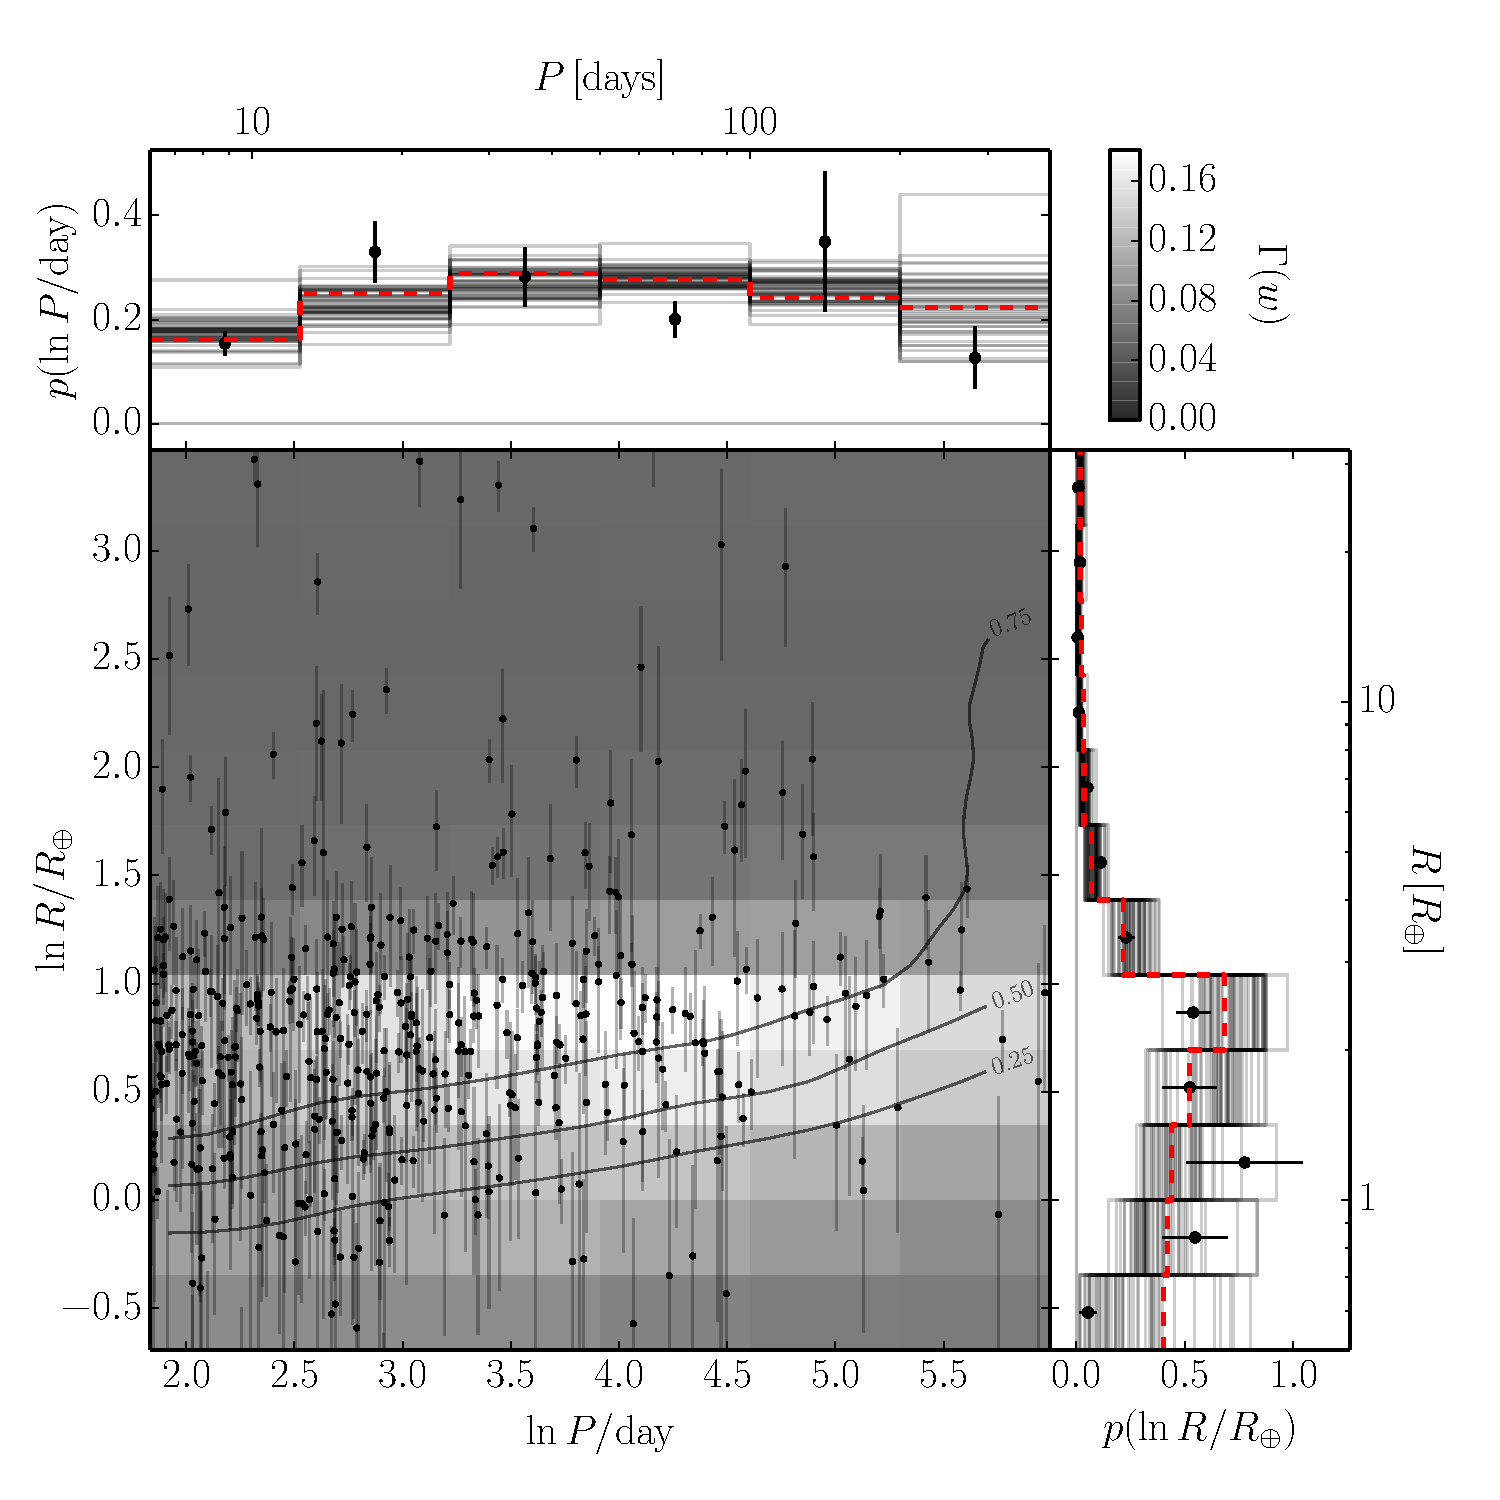
\includegraphics[width=\textwidth]{figures/simulation/results.pdf}
\end{center}
\caption{%
The same as \fig{smooth-results} for \modelb.
\dfmtodo{UPDATE THIS FIGURE TO FINAL VERSION}
\figlabel{simulation-results}}
\end{figure}

\section{Extrapolation to Earth}

As well as inferring the ocurrence distribution of exoplanets, this dataset
can also be used to constrain the rate of Earth analogs.
Even though no true analog has been observed, we can make some assumptions
about the distribution (as described below) and extrapolate to the location of
the Earth.
Explicitly, we constrain the rate of exoplanets \emph{evaluated at the
location of Earth}
\begin{eqnarray}
\gammaearth &=& \rate (\ln\period_\oplus,\,\ln\radius_\oplus) \\
&=&
\left.\frac{\dd N}{\dd\ln\period\,\dd\ln\radius}\right|
_{\radius=\radius_\oplus,\,\period=\period_\oplus}\quad.
\end{eqnarray}
This is also the quantity that \citet{petigura} estimated in different units.

\begin{figure}[p]
\begin{center}
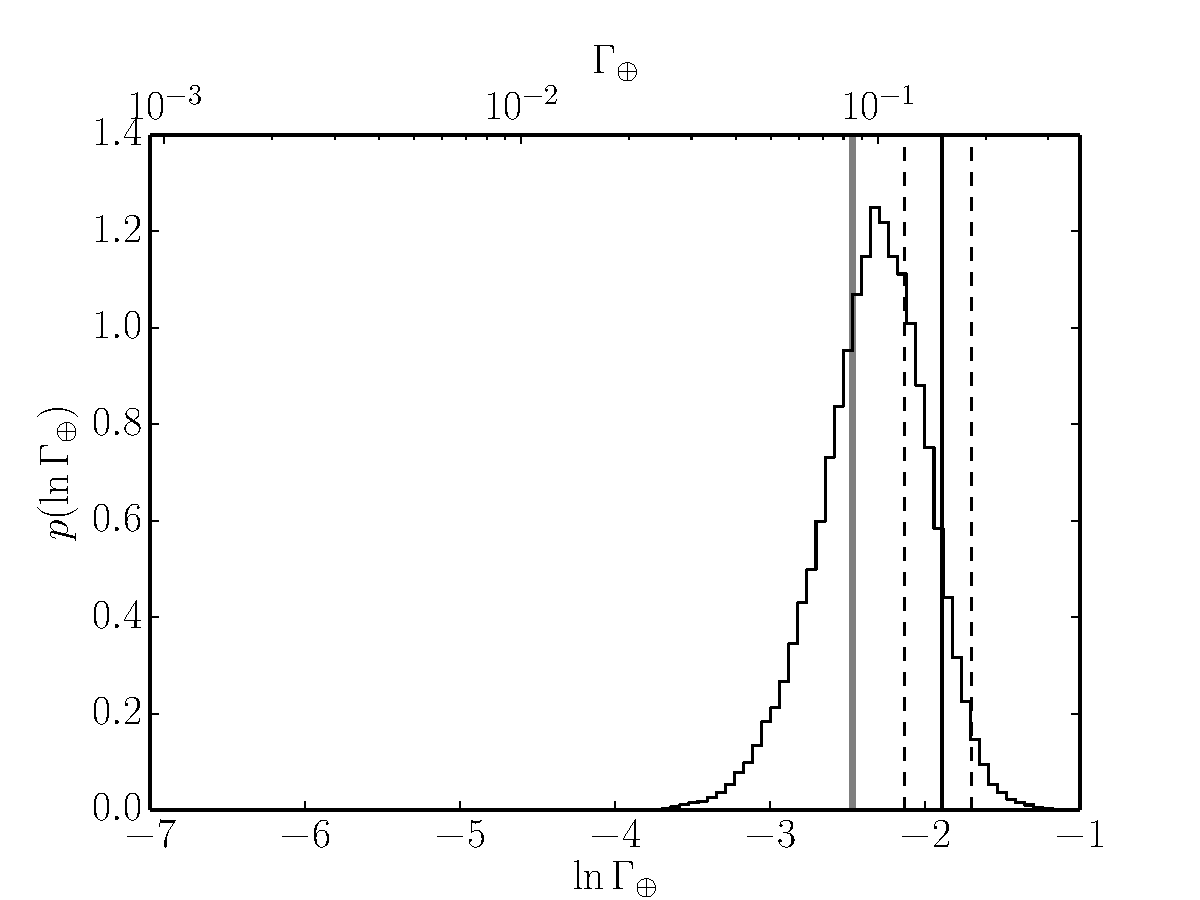
\includegraphics[width=0.6\textwidth]{figures/smooth/rate.pdf}
\end{center}
\caption{%
The extrapolated rate of Earth analogs \gammaearth\ as inferred by the
different techniques.
Applying the method used by \citet{petigura} gives a constraint indicated by
the vertical black line with error bars shown as dashed lines.
The histogram is the MCMC estimate of our posterior constraint on this rate
and the true value is indicated as the thick gray vertical line.
\figlabel{smooth-rate}}
\end{figure}

\begin{figure}[p]
\begin{center}
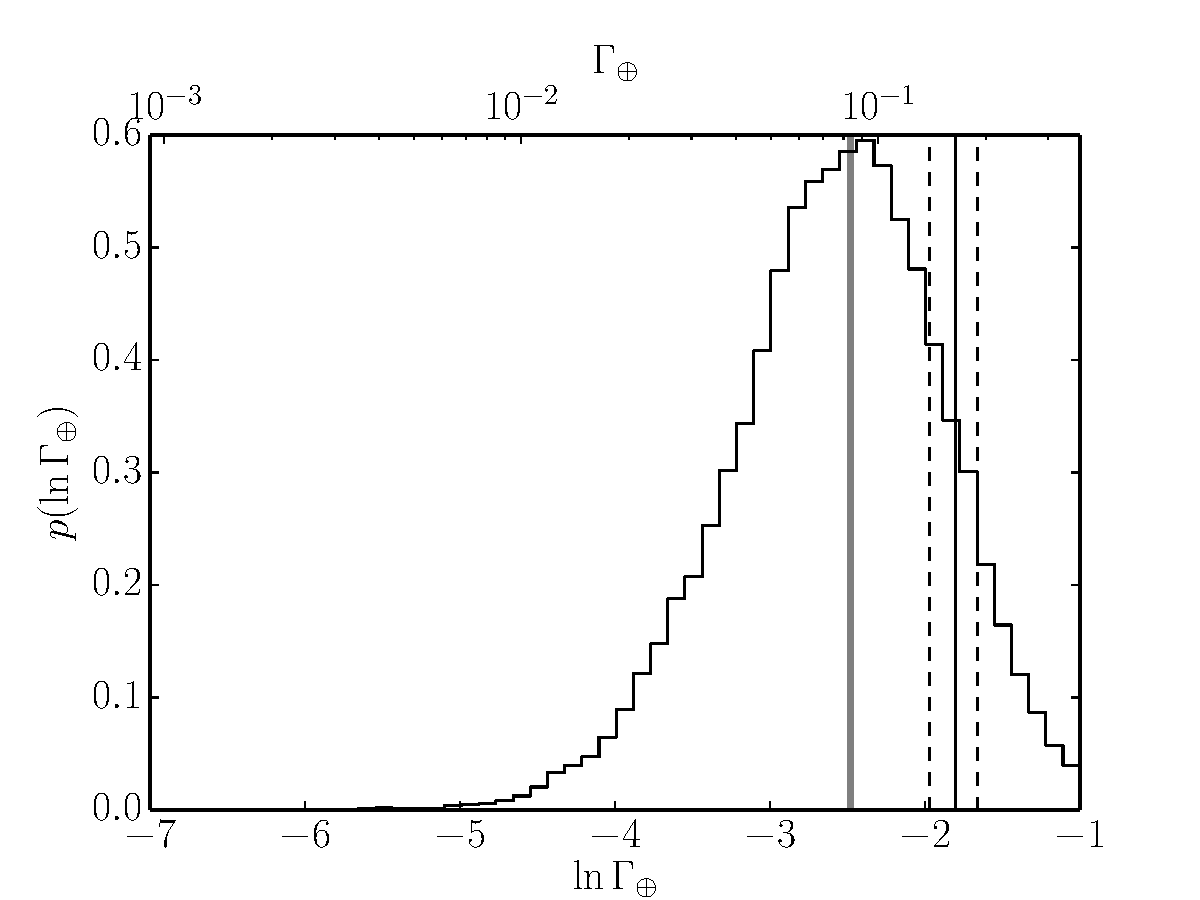
\includegraphics[width=0.6\textwidth]{figures/simulation/rate.pdf}
\end{center}
\caption{%
The same as \fig{smooth-rate} for \modelb.
\dfmtodo{UPDATE THIS FIGURE TO FINAL VERSION}
\figlabel{simulation-rate}}
\end{figure}

\section{Real data}

\begin{figure}[p]
\begin{center}
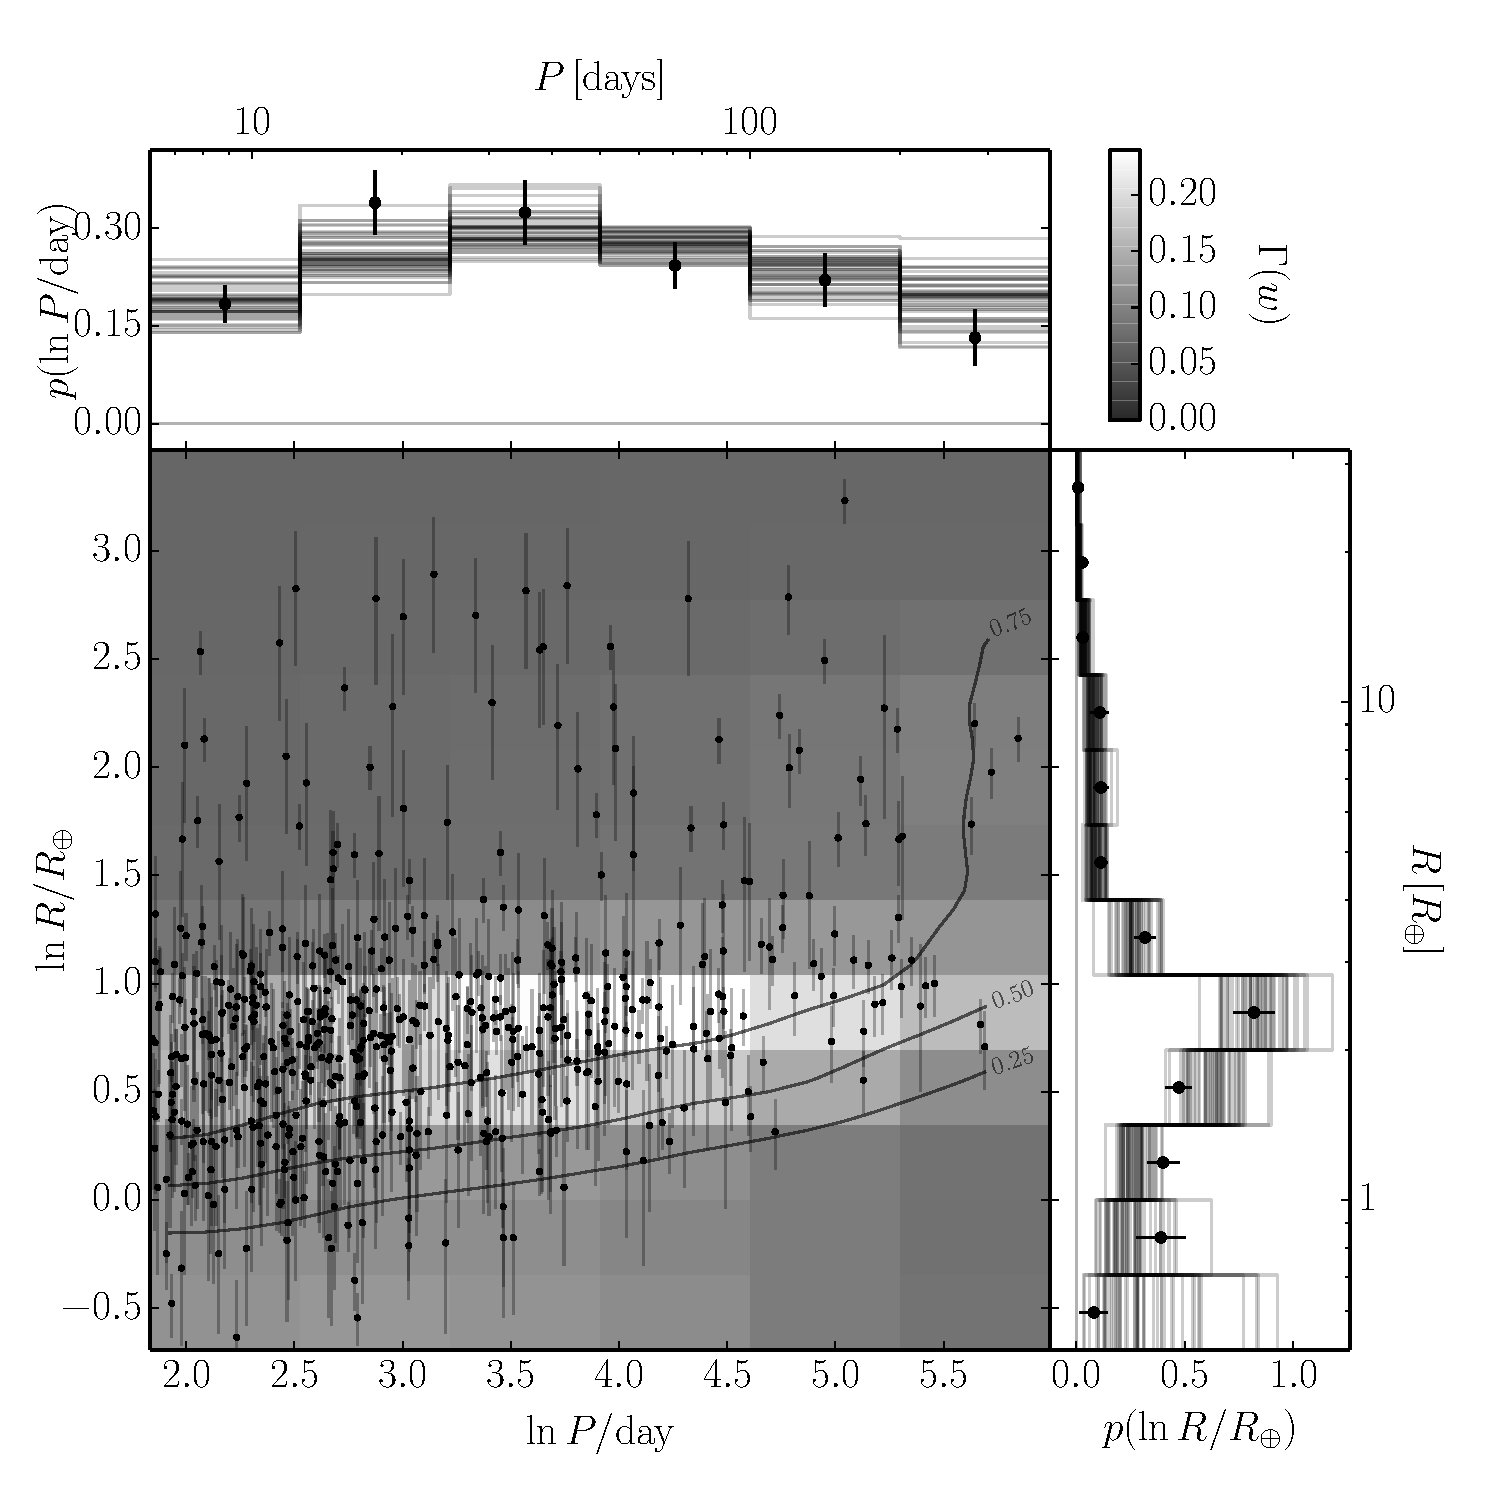
\includegraphics[width=\textwidth]{figures/results/results.pdf}
\end{center}
\caption{%
The same as \fig{smooth-results} when applied to the observed data from
\citet{petigura}.
\figlabel{real-results}}
\end{figure}

\begin{figure}[p]
\begin{center}
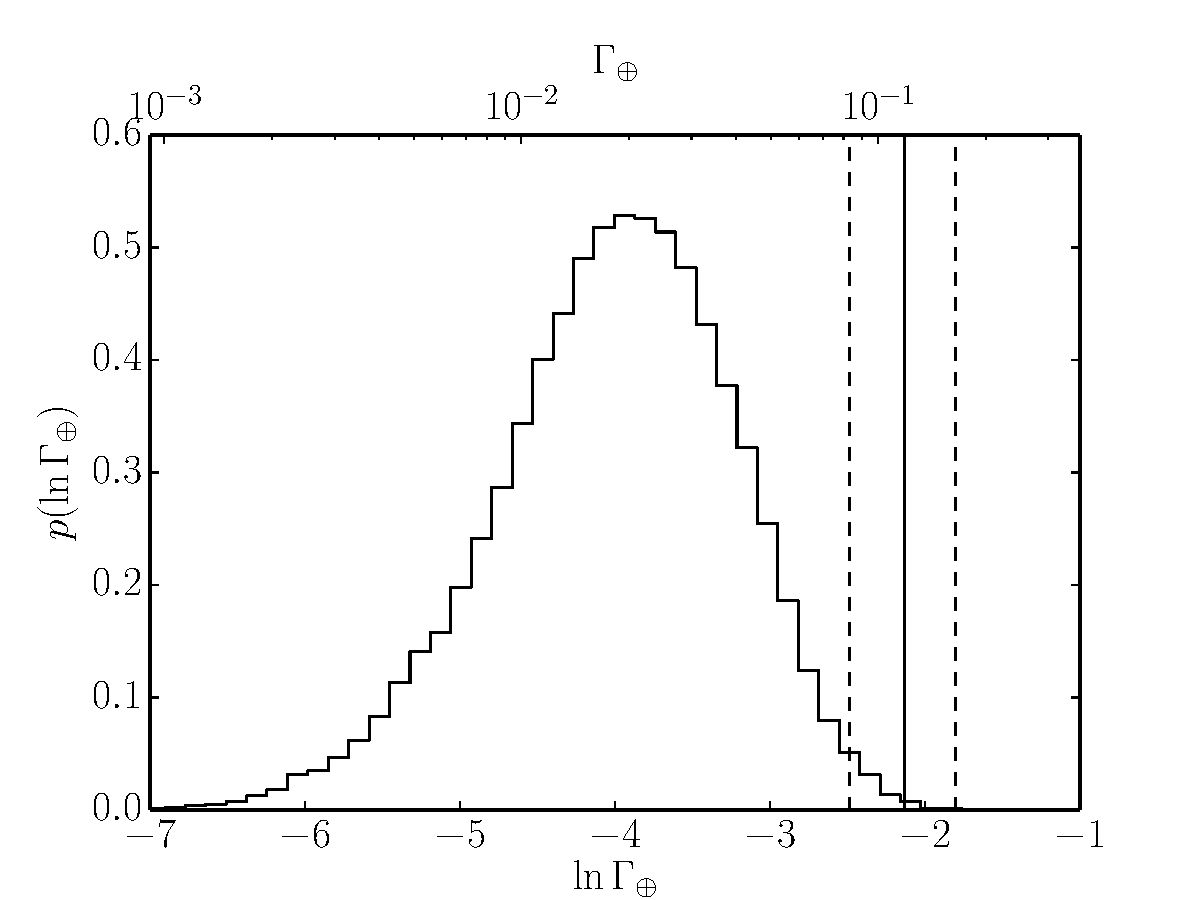
\includegraphics[width=0.6\textwidth]{figures/results/rate.pdf}
\end{center}
\caption{%
The same as \fig{smooth-rate} but applied to the catalog from \citet{petigura}.
\figlabel{real-rate}}
\end{figure}

\section{Discussion}

We have made the first measurement of the Earth-like exoplanet population that
is based on forward modeling, takes proper account of the observational
uncertainties on planet radii, and makes use of extremely flexible
non-separable distributions for period and radius.
We find \hoggtodo{BLAH BLAH BLAH.}

Although our method makes weaker assumptions than any previous work in this
area, of course it \emph{does} make strong assumptions.
It assumes that the data set (from \citealt{petigura}) contains planets and
only planets (no false positives).
It assumes that the individual-planet radius uncertainties are also correctly
determined.
It assumes that the completeness calculation (again from \citealt{petigura})
is accurate and smoothly varying with period and radius; it makes no attempt
to adjust the completeness star-by-star for brightness or variability.
It assumes that the exoplanets are all independently drawn from the same
distribution function, with no regard to age, metallicity, or multiplicity.

Although we have taken account of the radius uncertainties in a principled
way, we did make one important approximation: We ignored planets with central
values far outside the period and radius box in which we built the model.
That is, we assumed that there are no very large outliers in radius
determination.
This assumption is a complex one; it involves the effective, end-to-end error
distribution in the data set, but also smoothness of the distribution function
at or near the edges of the analysis box.

If our inferences are right about true Earth analogs, then we expect that
there are about XXX transiting Earth analogs hidden in the \kepler\ data set.
We would be able to find some of these Earth analogs if the effective noise
level in the data could be reduced by a factor of about XXX.
We have identified a number of directions along which this noise reduction
might happen, including but not limited to retrospective data-driven or
physics-driven recalibrations of the \kepler\ focal plane
(\citealt{hoggwhitepaper}), new methods for performing aperture photometry,
and better models for stochastic instrument variability or stochastic
intrinsic stellar variability that take account of frequency structure
(\citealt{brewer, carter, roberts}).
If any (or all) of these deliver substantial improvements for \kepler\
archival data reanalyses, it's Nobel Prize time!  (Or at least \textsl{The
Colbert Report}?)

All of the code used in this project is available from
\url{http://github.com/dfm/exopop} under the MIT open-source software license.
This code (plus some dependencies) can be run to re-generate all of the
figures and results in this \paper; this version of the paper was generated
with git commit \texttt{\githash} (\gitdate).

\acknowledgments
It is a pleasure to thank
    Erik Petigura (Berkeley),
    \etc
for helpful contributions to the ideas and code presented here.
This project was partially supported by the NSF (grant AST-0908357), and NASA
(grant NNX08AJ48G).
This research made use of the NASA \project{Astrophysics Data System}.

\appendix

\section{Maximum likelihood estimators for noiseless catalogs}
\sectlabel{histogram}

Equation XXXX gives the likelihood of a catalog $\catalog =
\{\entry_k\}_{k=1}^K$, conditioned on a particular choice of occurence rate
parameters \ratepars:
\begin{eqnarray}
\ln p(\catalog\,|\,\ratepars) &=& \sum_{k=1}^K \ln \rate(\entry_k)
    - \int \rate(\entry) \dd\entry \quad.
\end{eqnarray}
If we model the occurence rate as a piecewise constant function
\begin{eqnarray}
\rate (\entry) &=& \left \{\begin{array}{ll}
\ratepar_1 & \mathrm{if\,} \entry \in \binarea_1, \\
\cdots & \cdots \\
\ratepar_N & \mathrm{if\,} \entry \in \binarea_N, \\
0 & \mathrm{otherwise}
\end{array}\right.
\end{eqnarray}
where $\binarea_n$ is the volume of the bin $n$, the log likelihood becomes
\begin{eqnarray}
\ln p(\catalog\,|\,\ratepars) &=&
    \sum_{k=1}^K \sum_{n=1}^N \mathbf{1}[\entry_k \in \binarea_n]
        \ln\ratepar_n
    - \sum_{n=1}^N \ratepar_n\,\binarea_n \quad.
\end{eqnarray}
The maximum likelihood solution to this can be computed analytically
\begin{eqnarray}
\frac{\dd \ln p(\catalog\,|\,\ratepars)}{\dd \ratepar_m} &=&
    \frac{N_m}{\ratepar_m} - \binarea_m \\
\to \quad \ratepar_m &=& \frac{N_m}{\binarea_m}
\end{eqnarray}
where $N_m$ is the number of objects in the bin $m$.
This result is simply a \emph{normalized histogram} of the points.

Including the completeness function $\completeness(\entry)$ is as simple as
modeling the observable occurence rate as
\begin{eqnarray}
\rate (\entry) &=& \completeness(\entry) \, \left \{\begin{array}{ll}
\ratepar_1 & \mathrm{if\,} \entry \in \binarea_1, \\
\cdots & \cdots \\
\ratepar_N & \mathrm{if\,} \entry \in \binarea_N, \\
0 & \mathrm{otherwise}
\end{array}\right. \quad.
\end{eqnarray}
This leads to a similar analytic maximum likelihood solution
\begin{eqnarray}
\frac{\dd \ln p(\catalog\,|\,\ratepars)}{\dd \ratepar_m} &=&
    \frac{N_m}{\ratepar_m}
    - \int_{\binarea_m} \completeness(\entry)\dd\entry \\
\to \quad \ratepar_m &=& N_m \,
    \left [\int_{\binarea_m} \completeness(\entry)\dd\entry \right ]^{-1}
\end{eqnarray}
where the remaining integral is over the bin $m$.
This result is \emph{almost} the same as the inverse-detection-efficiency
procedure but each point is weighted by the bin-averaged efficiency instead of
the per-object efficiency.

\newcommand{\arxiv}[1]{\href{http://arxiv.org/abs/#1}{arXiv:#1}}
\begin{thebibliography}{}\raggedright

\bibitem[Adams, Murray \& MacKay(2009)]{poiss-gp}
Adams, R.~P., Murray, I., \& MacKay, D.~J.~C.\ 2009, ICML, 2009, 9
(\href{http://homepages.inf.ed.ac.uk/imurray2/pub/09poisson/}{online})

\bibitem[Brewer \& Stello(2009)]{brewer}
Brewer, B.~J., \& Stello, D.\ 2009, \mnras, 395, 2226 (\arxiv{0902.3907})

\bibitem[Carter \& Winn(2009)]{carter}
Carter, J.~A., \& Winn, J.~N.\ 2009, \apj, 704, 51 (\arxiv{0909.0747})

\bibitem[Dong \& Zhu(2013)]{dong}
Dong, S., \& Zhu, Z.\ 2013, \apj, 778, 53 (\arxiv{1212.4853})

\bibitem[Dressing  \& Charbonneau(2013)]{dressing}
Dressing, C.~D., \& Charbonneau, D.\ 2013, \apj, 767, 95 (\arxiv{1302.1647})

\bibitem[Gibson \etal(2012)]{gibson-gp}
Gibson, N.~P., Aigrain, S., Roberts, S., \etal\ 2012, \mnras, 419, 2683

\bibitem[Hogg \etal(2013)]{hoggwhitepaper}
Hogg, D.~W., Angus, R., Barclay, T., et al.\ 2013, \arxiv{1309.0653}

\bibitem[Hogg \etal(2010)]{hogge}
Hogg, D.~W., Myers, A.~D., \& Bovy, J.\ 2010, \apj, 725, 2166
(\arxiv{1008.4146})

\bibitem[Howard \etal(2012)]{howard}
Howard, A.~W., Marcy, G.~W., Bryson, S.~T., et al.\ 2012, \apjs, 201, 15
(\arxiv{1103.2541})

\bibitem[Lewis \& Shedler(1979)]{poisson}
Lewis, P.~A.~W., \& Shedler, G.~S.\ 1979, Naval Research Logistics Quarterly,
26, 403

\bibitem[Murray \etal(2010)]{ess}
Murray, I., Prescott Adams, R., \& MacKay, D.~J.~C.\ 2010, JMLR: W\&CP, 9, 541
(\arxiv{1001.0175})

\bibitem[Murray \& Prescott Adams(2010)]{ess-hyper}
Murray, I., \& Prescott Adams, R.\ 2010, Advances in Neural Information
Processing Systems, 23, 1723
(\arxiv{1006.0868})

\bibitem[Petigura \etal(2013a)]{petigura-a}
Petigura, E.~A., Marcy, G.~W., \& Howard, A.~W.\ 2013a, \apj, 770, 69
(\arxiv{1304.0460})

\bibitem[Petigura \etal(2013b)]{petigura}
Petigura, E.~A., Howard, A.~W., \& Marcy, G.~W.\ 2013b,
Proceedings of the National Academy of Science, 110, 19273 (\arxiv{1311.6806})

\bibitem[Rasmussen \& Williams(2006)]{gp}
Rasmussen, C.~E. \& Williams, C.~K.~I.\ 2006
Gaussian Processes for Machine Learning, MIT Press
(\href{http://www.gaussianprocess.org/gpml/}{online})

\bibitem[Roberts \etal(2013)]{roberts}
Roberts, S., McQuillan, A., Reece, S., \& Aigrain, S.\ 2013, \mnras, 435, 3639
(\arxiv{1308.3644})

\bibitem[Tabachnik \& Tremaine(2002)]{tabachnik}
Tabachnik, S., \& Tremaine, S.\ 2002, \mnras, 335, 151
(\arxiv{astro-ph/0107482})

\bibitem[Tremaine \& Dong(2012)]{tremaine}
Tremaine, S., \& Dong, S.\ 2012, \aj, 143, 94 (\arxiv{1106.5403})

\bibitem[Youdin(2011)]{youdin}
Youdin, A.~N.\ 2011, \apj, 742, 38 (\arxiv{1105.1782})

\end{thebibliography}

\end{document}
